%
%   Chapter Introduction
%
%   Qing-Cheng Li (r01922024 at csie dot ntu dot edu dot tw)
%   R.O.C.103.07
%
\chapter{緒論}
\label{c:intro}

近年來,隨著網際網路的快速發展,網際網路中開始出現越來越多彙整人類知識的網站與資源,
例如Wikipedia\footnote{http://www.wikipedia.org/},目前已經有超過280種語言,其中光是英語的條目就超過4,500,000條,
是透過來自世界各地的志願編輯者一字一句的貢獻建立而成的。

除了讓世界各地的人們可以在網際網路上共享知識之外,也讓計算機得以利用人類的知識,
輔助、改善、甚至自動化人工智慧、資料探勘與擷取、知識汲取、自動問答系統等任務。

為了達成此一目的,使計算機可以看懂人類的知識,於是,
便出現了各式各樣透過擷取網路上的知識資源,產生的結構化知識資料庫,甚至進一步並彼此相互鏈結。
如圖\ref{i:lod}所示,目前已有不少的結構化知識資料庫。

\begin{figure}
\centering
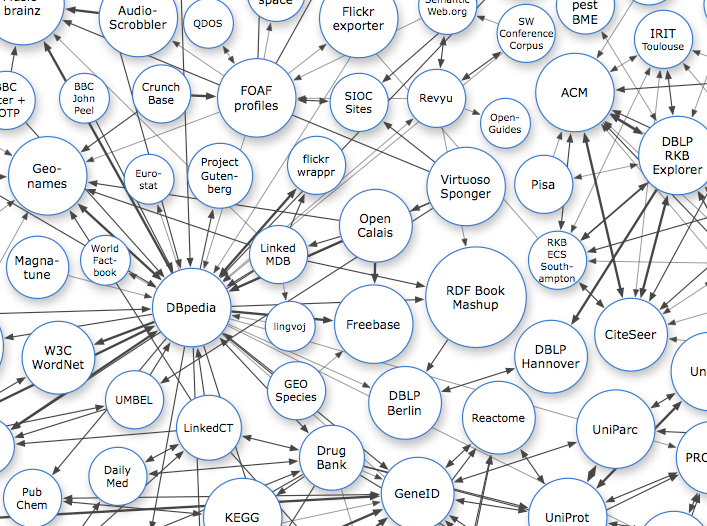
\includegraphics[width=0.5\textwidth]{images/01-lod-datasets}
\caption{結構化知識資料庫之間的鏈結}
\label{i:lod}
資料來源:linkeddata.org(2011)
\end{figure}

%
%   Background
%
\section{背景介紹}
在現今這個資訊社會,網際網路是重要的知識來源。當有新的事件發生時,
例如某人的出生或死亡、某政治人物贏得了選舉、某地發生了天災等等,
這些資訊便會在網路上透過網路新聞、網誌、論壇、社群網站、微網誌等管道流傳。
這代表著可能有新的知識出現了,或者舊有的知識發生了變動。
而一些知識資料庫如Wikipedia的志願編輯者注意到這些資訊之後,
便會據此更新Wikipedia上的條目,將這些新的知識加入資料庫之中。

這種用來儲存實體(Entity)與實體的特性(Properties)、
實體與實體間的關係(Relationships)的資料庫被稱為知識庫(Knowledge Base),
Wikipedia就是一個知識庫。

在Wikipedia之中,Wikipedia用文章(條目)的形式儲存了人物、組織、公司、城市、事件等實體,
文章透過超連結(Hyperlinks)互相鏈結,包含超連結的句子描述了實體與實體間的關係。
除此之外,還有的條目會包含資訊框(Infoboxes),以半結構化的形式描述了實體的特性,
圖\ref{i:wiki}就是一個Wikipedia條目的例子。
圖中的句子「... who was the co-founder, chairman, and CEO of \emph{Apple Inc}.」,
說明了Steven Jobs與Apple公司之間的關係:Jobs是Apple公司的CEO。
而這個關係對Jobs這個實體來說,亦代表其具有「was CEO of」的特性。
也就是說,與其他實體間的關係帶有實體特性的資訊。

\begin{figure}
\centering
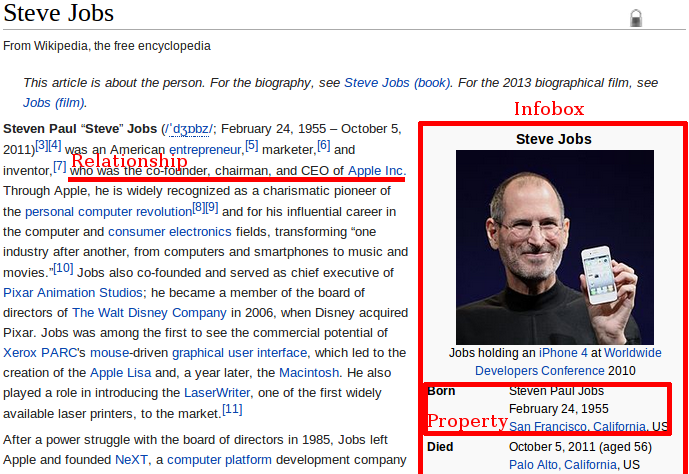
\includegraphics[width=0.65\textwidth]{images/01-wiki-as-kb}
\caption{Wikipedia條目與資訊框}
\label{i:wiki}
\end{figure}

除了Wikipedia之外,還有DBpedia \citep{dbpedia}、YAGO \citep{yago}、Freebase \citep{freebase}等規模大小不一、不同應用的知識庫。
其中YAGO、DBpedia是透過自動化的方法擷取Wikipedia的內容,Freebase仰賴社群更新,
這些知識庫都直接或間接仰賴志願者將新知識加入。

%
%   Motivation
%
\section{研究動機}
知識庫內所記載的知識直接或間接仰賴志願編輯者的維護與更新,
但這些人數比起資料庫中所需要維護的實體顯然非常的少。
這意味著知識庫的更新總是落後於新知識——無論是過去從來不知道的知識或是舊有知識內容的更動——的產生,
當新知識產生一段時日之後,知識庫的維護者才會更新知識庫。
\cite{kba2012}追蹤了約60,000個被Wikipedia引用的來源網頁,
計算從該網頁產生的時間與被Wikipedia引用的時間差,
如圖\ref{i:wikicitenews}所示,中位數約為一年,呈現了這種落後。
因此,如何讓人工編輯的速度可以跟上新知識出現的速度便成為一個重要的課題。

\begin{figure}
    \centering
    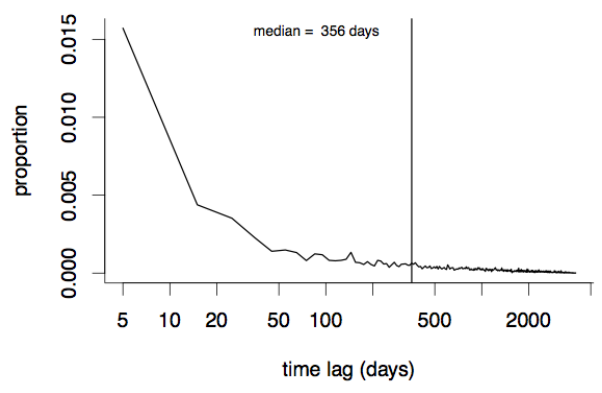
\includegraphics[width=0.65\textwidth]{images/01-wiki-cite-delay}
    \caption{Wikipedia引用延遲}
    \label{i:wikicitenews}
\end{figure}

為了縮短這個差距,自2012年起至今的每年美國NIST\footnote{National Institue of Standards and Technology}的TREC\footnote{Text Retriveal Conference}都會舉辦知識庫加速(Knowledge Base Acceleration, KBA)競賽,
提供了一個從由新聞、部落格、論壇等內容所組成、依時間所排列的龐大內容串流\footnote{2012年包含了4,973個小時,2013年包含了11,948小時。\citep{kba2013}每小時包含約100,000份文件。}(Content Strean),模擬真實世界中資訊的產生。
希望參賽者可以建立一個系統,這樣的內容串流中,
對有興趣的實體\footnote{2012年有27個人物、2個組織,2013年有98個人物,12個組織與24個設施。},
包含了人物、組織或建築,進行過濾,
推薦文件給知識庫的編輯者,建議編輯者這份文件可能含有新的知識可供更新知識庫。

要從可能包含新知識的內容串流中,過濾出可能可以協助更新知識庫的文件,
則需要知道文章中是否包含了我們關注的實體以及知識。
例如文章中出現了句子「Jobs was born in San Francisco, California on February 24, 1955」,
這其中就包含了「Jobs」、「San Francisco」、「California」等實體,
透過「was born in」這個樣式(Pattern),
可以知道「Jobs」與「San Francisco」、「California」間具有「出生於」的關係,
包含「出生地」這項實體特性。
若可以快速地辨識文章中是否包含這些資訊,
推薦給知識庫的編輯者參考,便能夠進一步地加速知識庫的更新與維護。

%
%   Goal
%
\section{研究目標}
本研究的目標是建立一個過濾系統,可以快速地處理內容串流。
對於內容串流內的每一份文件,偵測該文件中是否存在我們感興趣的實體特性。

本研究將利用樣式來判斷是否有實體間關係這樣的特性存在於文件之中,
也就是說,若有一個樣式與關係的資料庫,透過樣式比對,當文句比對成功時,
透過資料庫尋找對應的關係。

整個偵測的過程要有效率和有效能。
這個系統要有效率,如果樣式比對或對句子進行更深入的剖析的效率不高,
就沒有辦法處理內容串流大量的文件。
這個系統要有效能,而透過樣式判斷關係的效能可能會受到樣式本身的品質(Quality)、
樣式的覆蓋度(Coverage)、樣式值得信賴的程度(Reliability)、
樣式-關係對映的歧義問題(Ambiguity)等因素影響。

透過這個系統,我們將知道經過過濾的文件到底是完全沒有提及我們感興趣的實體特性,
還是提到一個,甚至多個實體特性。
有這樣的資訊就可以進行更進一步的分析,
例如這個特性是屬於哪個實體的?這個特性的內容是什麼?
來判斷是不是應該要對實體的特性內容進行更新,甚至是自動更新,
以幫助知識庫的更新與維護。

%
%   Structure
%
\section{論文架構}
本論文共分成五個章節。
第一章是緒論,簡介本研究的背景、動機與目標。
第二章是相關研究與文獻,列舉了與知識庫相關的研究與資源以及關係與樣式相關的研究。
第三章是研究方法,提出如何於內容串流中究偵測實體特性的方法與步驟。
第四章是實驗結果與分析,說明實驗資料集、評估方式與結果分析。
第五章是結論與未來展望,總結研究成果。
